\section{Phase 2: Point of Order!}

\noindent \textbf{Timeline: October 2 -- November 20, 2025}

The mission of Phase 2 was to transmute raw inputs into the definitive \texttt{pienza.db} warehouse. While retrospectively structured as a logical progression, the execution followed a complex, non-linear trajectory defined by recursive discovery loops.

The initial architecture (Contextual Features $\to$ ETL $\to$ DB) was stress-tested by a preliminary EDA, which exposed critical latent flaws—specifically systemic geospatial corruption and the absence of state-dependent context. This necessitated a "Rollback and Refine" protocol: retreating from exploratory analysis to execute deep geospatial remediation (Phase 2B) and advanced contextual engineering (Phase 2C). 

Only after these intelligence layers were stabilized was the final, structural consolidation executed (Phase 2D). This iterative campaign culminated in the deployment of an \textbf{Idempotent ETL Pipeline}, capable of regenerating the entire database from source in a single, reproducible run.

% --- SUB-PHASE A ---
\subsection{Phase 2A: Contextual Feature Synthesis}

Having officially transitioned from the Acquisition into the Engineering Phase, the primary mandate was to continue extracting high-fidelity signal from the raw OCR logs. These represent the second set of contextual features and are integrated directly into the \texttt{offers} table, completing the static snapshot of each decision event.


\subsection{Incentive Deconstruction}
The \texttt{special\_note} field from the raw OCR ingestion arrived as a high-entropy text blob containing compounded operational metadata (e.g., \textit{Surge, Turbo+, VIP status, Reservations}). To transform this into predictive features, a modular deconstruction engine was architected using a suite of Regular Expressions (Regex).

\subsubsection{Regex Parsing Architecture}
The engine was designed to isolate binary flags and extract continuous numerical values for specific incentive tiers. This process involved handling multilingual syntax (Spanish/English) and non-standard character encoding, such as the \texttt{CHAR(160)} non-breaking space, which frequently disrupted standard string splitting.

\begin{table}[H]
    \centering
    \scriptsize % Smaller font to fit the increased data density
    \begin{tabularx}{\textwidth}{l l X}
        \toprule
        \textbf{Category} & \textbf{Feature (Boolean / Amount)} & \textbf{Regex Logic (Simplified)} \\
        \midrule
        \multirow{4}{*}{\textbf{Incentives}} 
        & \texttt{is\_turbo\_plus} / \texttt{amount} & \texttt{(?i)((?:Turbo\textbackslash+.*?[\textbackslash d\textbackslash .]+)|(?:[\textbackslash d\textbackslash .]+.*?turbo fare))} \\
        & \texttt{is\_surge} / \texttt{amount} & \texttt{(?i)(Surge.*?[\textbackslash d\textbackslash .]+ | fare includes a surge...)} \\
        & \texttt{is\_priority} / \texttt{amount} & \texttt{(?i)((?:priority|prioritario).*?[\textbackslash d\textbackslash .]+ | ...priority trip start)} \\
        & \texttt{is\_reservation} / \texttt{amount} & \texttt{(?i)res.*?(\textbackslash d+\textbackslash .\textbackslash d+|\textbackslash d+)} \\
        \midrule
        \multirow{3}{*}{\textbf{Trip Attributes}} 
        & \texttt{is\_long\_trip} & \texttt{(?i)\textbackslash b(long|largo)\textbackslash b} \\
        & \texttt{is\_multiple\_destinations} & \texttt{(?i)\textbackslash w*dest\textbackslash w*} \\
        & \texttt{is\_teens} & \texttt{(?i)Teens} \\
        \midrule
        \multirow{5}{*}{\textbf{Rider Metadata}} 
        & \texttt{is\_vip} & \texttt{(?i)(VIP|Rider is VIP|user is a VIP)} \\
        & \texttt{is\_exclusive} & \texttt{(?i)(Exclusivo|Exclusive)} \\
        & \texttt{is\_identity\_verified} & \texttt{(?i)(Identidad verificada|Identity verified)} \\
        & \texttt{rider\_star\_rating} & \texttt{(\textbackslash d+\textbackslash .\textbackslash d+|\textbackslash d+)} \\
        & \texttt{rider\_reviews} & \texttt{\textbackslash ((\textbackslash d+)} \\
        \bottomrule
    \end{tabularx}
    \caption{Comprehensive deconstruction schema for the \texttt{special\_note} high-entropy field.}
    \label{tab:regex_logic}
\end{table}


% In 02_engineering.tex -> Section 3.6.2
\subsubsection{Generative Variability and Remediation}
During a subsequent EDA phase, a systemic inconsistency was identified regarding incentive classification. While the ingestion script was strictly sequential, the \textbf{generative extraction layer} exhibited non-deterministic behavior. Varying levels of model ``creativity'' across processing batches led to the conflation of \textit{Surge} and \textit{Turbo+} labels.

For instance, the model occasionally produced compounded, hallucinated strings such as: \textit{``Turbo+ of \$16.00 and Turbo+ of \$14.07 are included...''} These unstructured artifacts rendered standard Regex parsing insufficient. Because these discrepancies threatened the integrity of downstream profitability analysis, a second iteration of \textbf{Manual Remediation} was executed. The Agent performed a line-by-line audit, cross-referencing corrupted records against the original image assets to ensure 100\% data purity for the final training set.

\subsubsection{Technical Retrospective}
This cleaning phase yielded critical engineering insights regarding the extraction of structured data from visual UI elements via LLMs:
\begin{itemize}
    \item \textbf{Downstream Fragility:} Text parsing via Regex is highly susceptible to the non-deterministic variability of LLM-based OCR outputs. A single word change in the model's response can break a production pipeline.
    \item \textbf{Upstream Visual Mapping:} A superior architecture involves \textit{Visual Semantic Instruction} during the ingestion phase. Instructing the Vision model to distinguish incentives based on UI iconography (e.g., mapping the ``Lightning Bolt'' icon directly to a \texttt{surge\_amount} key) and requiring a strictly typed JSON output eliminates the need for ``artisanal'' post-processing.
\end{itemize}



\subsection{Chronology Features: Modeling Shift Progression}
To capture the impact of endgame decision-making, features were engineered to model an offer’s position within a discrete work session.

\subsubsection{The Offer Window Constraint}
For analytical consistency, a work session is defined by its \textbf{Offer Window}—the duration between the inaugural offer and the terminal offer of a shift—rather than total physical operational time. To prevent \textbf{Label Contamination}, the window was programmatically truncated 15 minutes prior to the Agent’s arrival its home base. This ensures that the dataset minimizes "terminal rejections" where the agent had no real intent of accepting any ride whatsoever. Two primary features were calculated to quantify temporal positioning:
\begin{itemize}
    \item \textbf{\texttt{time\_in\_session\_sec}:} The elapsed time between the current offer and the session's first recorded offer.
    \item \textbf{\texttt{session\_progress\_ratio}:} A normalized metric ranging from 0.0 (first offer) to 1.0 (final offer). This feature is the primary proxy for the agent's psychological state during the "Endgame" phase. It allows the model to learn the collapsing acceptance threshold for non-homecoming vectors as the ratio approaches 1.0.
\end{itemize}


\subsection{Trajectory Intelligence: Localization Trials}
While the \texttt{offers} table successfully captured the coordinates for pickup and dropoff points, the Agent’s own physical location at the moment of the offer remained unrecorded. Although the Agent possessed subjective ground truth from field experience, this spatial context was missing from the structured dataset. Recognizing that the Agent's relative position is a high-value predictor for decision modeling, a series of four localization experiments were conducted to infer this latent variable.

\subsubsection{Trial 1: External Telemetry (Google Location History)}
\textbf{Status: Failed.} Initial attempts were made to utilize the \texttt{location-history.json} export from Google Takeout. However, the device configuration during the acquisition phase was restricted to "While Using" rather than "Always," resulting in a truncated and inconsistent dataset. The lack of continuous polling rendered this external source insufficient for high-precision temporal alignment.

\subsubsection{Trial 2: Geometric Inference (Trilateration)}
\textbf{Status: Investigatory.} This protocol attempted to infer location using only the data within the offer card (\textit{Distance to Pickup}). By identifying clusters of three or more concurrent offers, the system utilized the \texttt{distance\_to\_pickup} as a radius for a trilateration optimization algorithm (\texttt{SciPy.optimize.minimize}) to find the agent's most probable coordinate. This approach was ultimately rejected due to platform-level address obfuscation. Without precise centroids for the circles, the optimization results deviated significantly from operational reality.

\subsubsection{Trial 3: Linear Temporal Interpolation (Phase 2 Baseline)}
\textbf{Status: Ratified.} A robust internal baseline was developed leveraging the verified coordinates of accepted trips ($T_0 \dots T_4$) as high-fidelity anchors. Initial implementations executed interpolation across a continuous timeline. This "session-blindness" caused offers occurring between distinct shifts (e.g., overnight gaps) to be interpolated across massive temporal distances, generating physically impossible vectors.

\medskip
To ensure physical plausibility, the interpolation logic (\texttt{pandas.merge\_asof}) was re-architected with a strict \texttt{by='session\_id'} constraint. This mathematically guaranteed that the "before" and "after" anchors for any given offer were selected exclusively from within the same operational session, permanently eliminating the teleportation error.

\subsubsection{Trial 4: Home Vector Alignment (Strategic Extension)}
\textbf{Status: Final Champion (Post-Phase 2).} This methodology involved calculating the \textbf{Cosine Similarity} between the \textit{Movement Vector} (Agent $\to$ Dropoff) and a fixed \textit{Home Vector} (Agent $\to$ \textit{Anzures}). While this feature eventually became the dominant spatial predictor, the project relied on the Trial 3 Interpolation baseline for the duration of the Phase 2 structural engineering. This feature successfully quantified the Agent’s session-termination behavior.



\subsection{High-Precision Temporal Recovery}
Standard minute-level timestamps (HH:MM) proved insufficient for analyzing high-frequency market dynamics. To recover seconds-level precision, a custom Python pipeline was developed to extract internal metadata from the non-standard PNG chunks of the source assets. 

This timing capability was identified during the localization trials, as the investigation initially sought to retrieve GPS metadata from the image assets. While geospatial data was absent, the discovery of second-level markers enabled a higher analytical resolution. Two primary architectural risks necessitated this precision: iOS filename recycling and system-level offer repetition. The system often resends identical offers, creating visually congruent artifacts. As these repetitions can occur within a single minute but at distinct second intervals, standard HH:MM granularity would result in data loss through erroneous duplicate detection. To ensure uniqueness, a primary key, \texttt{event\_id}, was generated via a SHA-256 hash of a combined event signature:

\begin{equation}
    event\_id = \text{SHA-256}(\text{image\_content\_hash} + \text{high\_precision\_timestamp})
\end{equation}

This transformed the unstructured file repository into an audited relational ledger. The resulting high-fidelity temporal baseline unlocked the engineering of velocity-based features from Phase 2D.




\subsection{The Canonical Version of the \texttt{offers} Table}
The following table represents the canonical version of \texttt{offers} prior to the ETL process into \texttt{pienza.db}.

\begin{table}[H]
    \centering
    \scriptsize
    \begin{tabularx}{\textwidth}{l p{7.5cm} l}
        \toprule
        \textbf{Logical Domain} & \textbf{Engineered Columns} & \textbf{Role} \\
        \midrule
        \textbf{Identity} & \texttt{offer\_id}, \texttt{session\_id}, \texttt{image\_content\_hash} & Traceability \\
        \midrule
        \textbf{Temporal} & \texttt{offer\_timestamp}, \texttt{time\_in\_session\_sec}, \texttt{session\_progress\_ratio} & Chronology \\
        \midrule
        \textbf{Physics} & \texttt{upfront\_fare}, \texttt{product\_category} & Financials \\
                         & \texttt{time\_to\_pickup\_sec}, \texttt{dist\_to\_pickup\_km} & Logistics (Pickup) \\
                         & \texttt{est\_trip\_time\_sec}, \texttt{est\_trip\_dist\_km} & Logistics (Trip) \\
        \midrule
        \textbf{Geospatial} & \texttt{pickup\_address}, \texttt{dropoff\_address} & Raw Geodata \\
                            & \texttt{pickup\_lat/lon}, \texttt{dropoff\_lat/lon} & Absolute Location \\
                            & \texttt{inferred\_agent\_lat/lon/bearing/speed\_mps} & Agent Vector \\
                            & \texttt{interpolation\_quality}, \texttt{is\_imputed} & Data Integrity \\
        \midrule
        \textbf{Incentives} & \texttt{is\_surge}, \texttt{surge\_amount} & Dynamic Pricing \\
                            & \texttt{is\_turbo\_plus}, \texttt{turbo\_plus\_amount} & Strategic Bonus \\
                            & \texttt{is\_reservation}, \texttt{reservation\_amount} & Scheduling Fee \\
                            & \texttt{is\_priority}, \texttt{priority\_amount} & Demand Fee \\
        \midrule
        \textbf{Service Flags} & \texttt{is\_exclusive}, \texttt{is\_vip}, \texttt{is\_identity\_verified} & Client Tiering \\
                               & \texttt{is\_long\_trip}, \texttt{is\_multiple\_destinations}, \texttt{is\_teens} & Operation Complexity \\
        \midrule
        \textbf{Rider Profile} & \texttt{rider\_star\_rating}, \texttt{rider\_trip\_count} & Risk Metrics \\
        \midrule
        \textbf{Decision}      & \texttt{offer\_action}, \texttt{reason\_primary} (Target Variable) & Behavioral Data \\
                               & \texttt{heuristic\_flag}, & Strategic Context \\
                               & \texttt{driver\_state\_at\_request}, \texttt{outcome} & Operational State \\
        \midrule
        \textbf{Audit Layer}   & \texttt{special\_note\_raw}, \texttt{comment\_1}, \texttt{comment\_2}, \texttt{record\_status} & Forensics \\
        \bottomrule
    \end{tabularx}
    \caption{Canonical \texttt{offers} schema state at the conclusion of the initial engineering phase.}
    \label{tab:fact_table}
\end{table}




\subsection{Phase 2B: Geospatial Bottleneck}


Initial ingestion revealed systemic coordinate errors affecting $\approx 12.8\%$ of the dataset. A visual audit identified two primary failure modes: \textbf{Out-of-Bounds (OOB) Errors}, where ambiguous API requests placed coordinates outside the country (e.g., \textit{Santa Fe} resolving to New Mexico, or \textit{Terminal 2, Col. Peñón de los Baños} resolving to Guanajuato instead of the AICM zone), and \textbf{Artificial Singularities}, where distinct addresses collapsed into default centroids by the API.

To correct the OOB errors, a containerized filtration script was executed specifically over the list of anomalous records, enforcing a strict bounding box for Mexico City ($19.0, -99.5$ to $19.8, -98.7$). Subsequent geocoding requests were forced into this regional bias.

To resolve the singularities, a geometric engine was developed using the \texttt{osmnx} road network graph. The goal was to implement a linear jittering protocol to distribute points along the true geometry of target streets. 

As shown in Figure \ref{fig:remediation_maps}, the engine isolated street-level \textit{LineStrings} from their initial centroids. However, deployment confirmed that a fixed search radius was fundamentally contingent on \textbf{street length}. A small buffer effective for short segments proved insufficient for arterial routes or major avenues (\textit{e.g., Masaryk, Homero}). This created a cycle of diminishing returns where optimizing the radius for one street-type introduced errors into others, requiring constant manual overrides.

\begin{figure}[H]
     \centering
     % Row 1: Santa Fe
     \begin{subfigure}[b]{0.45\textwidth}
         \centering
         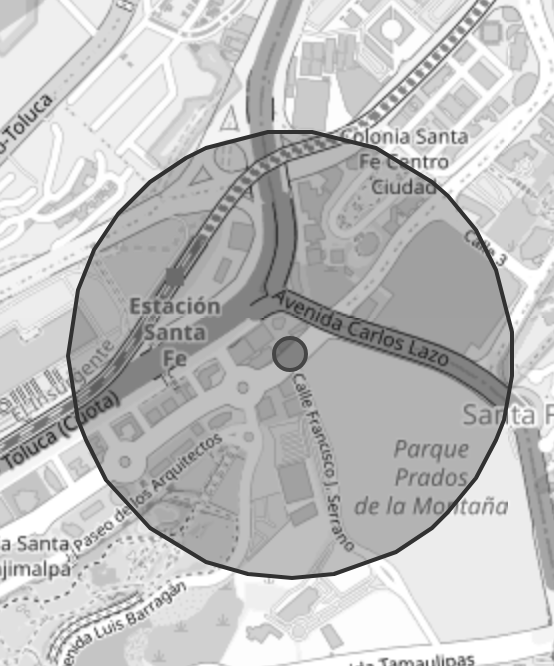
\includegraphics[width=\textwidth]{fig_sf_buffer.png}
         \caption{Ave. Santa Fe: Default Centroid}
     \end{subfigure}
     \hfill
     \begin{subfigure}[b]{0.45\textwidth}
         \centering
         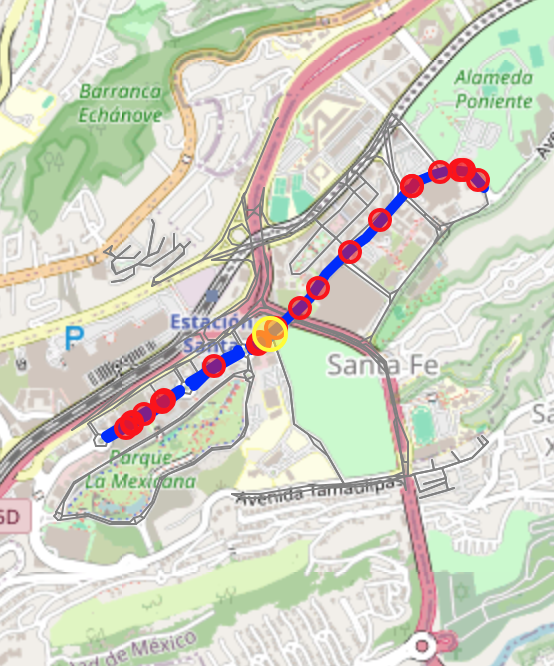
\includegraphics[width=\textwidth]{fig_sf_linear.png}
         \caption{Ave. Santa Fe: Linear Jittering}
     \end{subfigure}
     \vspace{0.3cm}
     % Row 2: Condesa
     \begin{subfigure}[b]{0.45\textwidth}
         \centering
         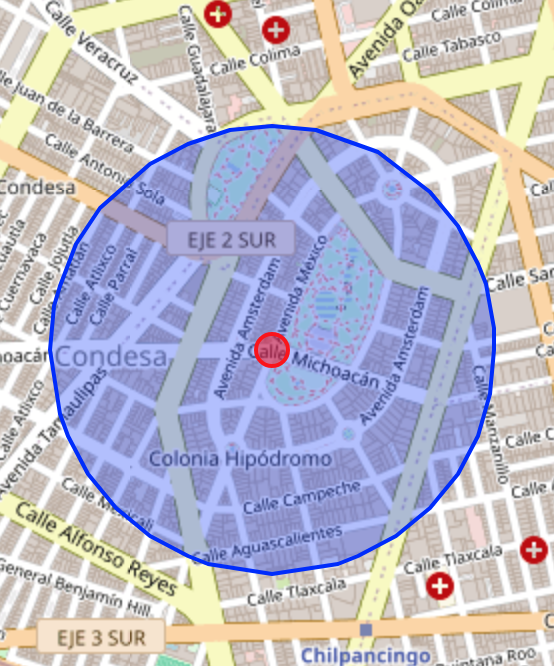
\includegraphics[width=\textwidth]{fig_condesa_buffer.png}
         \caption{Ave. Mexico: Default Centroid}
     \end{subfigure}
     \hfill
     \begin{subfigure}[b]{0.45\textwidth}
         \centering
         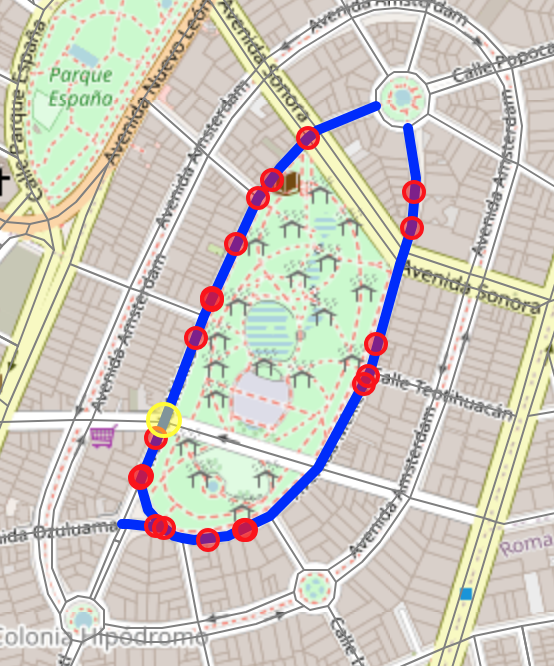
\includegraphics[width=\textwidth]{fig_condesa_linear.png}
         \caption{Ave. Mexico: Linear Jittering}
     \end{subfigure}
        \caption{Geospatial Reconciliation Results. The left column illustrates the default API centroids (Artificial Singularities). The right column represents the remediation protocol, randomizing coordinates across the true \textit{LineString} geometry.}
        \label{fig:remediation_maps}
\end{figure}

Upon identifying the limits of automated matching, the project prioritized analytical velocity over synthetic perfection. Since the \textit{dropoff} (destination) is the primary driver of the decision policy and the ambiguous set within that quadrant was statistically small ($\approx 310$ observations), the existing noise was determined to be acceptable. The project accepted the verified centroids for the contextual \textit{pickup} data to maintain development speed.

\begin{table}[H]
    \centering
    \small
    \begin{tabularx}{\textwidth}{l l r}
        \toprule
        \textbf{Quadrant} & \textbf{Nature} & \textbf{Observations} \\
        \midrule
        \texttt{dropoff\_unambiguous} & High-Precision Ground Truth & $\approx 4,325$ \\
        \addlinespace
        \texttt{dropoff\_ambiguous} & Managed Operational Noise & $\approx 310$ \\
        \addlinespace
        \texttt{pickup\_ambiguous} & Contextual Noise (Sufficient Precision) & $\approx 4,265$ \\
        \addlinespace
        \texttt{pickup\_unambiguous} & Standard Operational Signal & $\approx 500$ \\
        \bottomrule
    \end{tabularx}
    \caption{Geospatial integrity census post-remediation.}
    \label{tab:geo_quadrants}
\end{table}

\noindent \textit{Outcome: The dataset was geographically bounded to the operating area of Mexico City. By managing the noise floor, the project preserved the integrity of mission-critical destination features for the subsequent analytical phases.}


\subsection{Phase 2C: Stateful Intelligence}

While the physical parameters of an individual offer define a potential transaction, they fail to capture the broader operational context that governs an agent’s decision boundary. An agent's risk tolerance and profitability thresholds are dynamic functions of the current session's history—including accumulated fatigue, recent financial yield, and immediate market volatility. To bridge this gap, the project engineered a suite of stateful, session-dependent features.

These features were implemented through a custom Google Apps Script (\texttt{code.gs}) designed to operate as a sequential state machine. This engine iterates through the chronologically sorted dataset, maintaining a persistent "memory" of the agent's state across five critical dimensions:

\begin{enumerate}
    \item \textbf{Temporal Integrity (The No Look-Ahead Rule):} To prevent \textit{Data Leakage}, the engine strictly adheres to a temporal firewall. Features modeling past performance—such as the \texttt{cycle\_rolling\_avg\_spread}—only incorporate data from missions officially completed \textit{prior} to the current offer's timestamp.
    
   \item \textbf{Total Uncompensated Load:} The engine calculates \texttt{total\_accumulated\_deadhead\_sec}, aggregating the full non-revenue burden of the current cycle: \textit{Looking for rides} (T0) + \textit{Driving to Pickup} (T1) + \textit{Waiting for Passenger} (T2). This metric quantifies the accumulating "sunk cost" pressure on the agent's decision boundary.
    
    \item \textbf{Market Physics \& Dynamics:} Utilizing high-fidelity timestamps, the script calculates high-velocity signals such as \texttt{offer\_density}. A continuous \textbf{Traffic Index} is derived by normalizing trip duration against a baseline velocity of 120s/km, providing a scalar metric of congestion friction.

    \item \textbf{North Star Convergence:} The engine implements a \textbf{\$200 MXN} realized Earnings Per Hour (EPH) baseline as the Agent's "North Star." A suite of normalized indices (\texttt{eph\_*\_index}) quantifies how each offer deviates from this target, allowing the model to learn the agent's strategy of selecting rides that force the session mean to converge on this value despite individual variance. This enables the model to detect how the agent's multidimensional decision logic aligns towards forcing long-term convergence on this objective goal, even when individual sessions or offers are suboptimal.

    \item \textbf{The Profitability Funnel (Yield Analysis):} To quantify the delta between the platform's presentation and operational reality, EPH is calculated at four levels of granularity:
    \begin{itemize}
        \item \textbf{Direct:} Upfront Fare / Est. Trip Time. (The raw platform signal).
        \item \textbf{Operational:} Adjusted for \texttt{Time\_to\_Pickup}. 
        \item \textbf{Realized:} Realized Fare / Est. Trip Time. (Accounting for financial spread).
        \item \textbf{Complete:} Realized Fare / (\texttt{Total\_Accumulated\_Deadhead} + Est. Trip Time). (The holistic yield).
    \end{itemize}
    This funnel quantifies the Information Asymmetry gap where high-nominal offers may resolve as low-yield operations.
\end{enumerate}
\vspace{0.3cm}
\noindent \textbf{Technical Note on Model Integrity (\texttt{\_ML} vs \texttt{\_EDA}):}
A rigorous distinction is maintained between suffixes. Features intended for Supervised Learning (\texttt{\_ML}) are engineered using only historical averages available at the moment of decision. Features incorporating actual outcomes (\texttt{\_EDA}) are firewalled for exploratory analysis only, ensuring zero data leakage in the predictive engine.

\subsubsection{The Canonical Stateful Features}
These features were engineered within the \texttt{engineered\_features} table to provide the model with a stateful representation of the market and the agent's internal progress.

\begin{table}[H]
    \centering
    \scriptsize
    \begin{tabularx}{\textwidth}{l l X}
        \toprule
        \textbf{Dimension} & \textbf{Feature Name} & \textbf{Engineering Logic \& Strategic Proxy} \\
        \midrule
        \multirow{3}{*}{\textbf{Market Pressure}} 
        & \texttt{time\_since\_last\_offer} & Seconds elapsed since previous request. Proxy for market ``silence.'' \\
        & \texttt{offer\_density\_[10-180]sec} & Rolling counts of offers across 10, 30, 60, 180s windows. \\
        & \texttt{consecutive\_rejects} & Stateful counter resetting on acceptance. Proxy for frustration/patience. \\
        \midrule
        \multirow{5}{*}{\textbf{Supply \& Traffic}} 
        & \texttt{traffic\_index\_base\_120} & Normalized congestion metric (Baseline: 120s/km). Values $>1.0$ indicate friction. \\
        & \texttt{cycle\_avg\_dtp\_km} & Mean Distance-to-Pickup in current cycle. High values = Low local supply. \\
        & \texttt{cycle\_std\_dtp\_km} & Standard deviation of DTP. Measures supply volatility. \\
        & \texttt{cycle\_ttp\_dtp\_ratio} & Ratio of Pickup Time to Pickup Distance. Localized traffic proxy. \\
        & \texttt{dispatch\_lead\_time\_sec} & Time remaining on active trip when next offer is received (Chained Logic). \\
        \midrule
        \multirow{3}{*}{\textbf{Internal State}} 
        & \texttt{total\_acc\_deadhead\_sec} & Cumulative unpaid seconds (Search + Pickup + Waiting) in current cycle. \\
        & \texttt{cycle\_rolling\_avg\_spread} & Temporally-safe rolling average of the Upfront/Realized fare delta. \\
        & \texttt{cycle\_cum\_net\_earnings} & Cumulative realized income for the session. \\
        \midrule
        \multirow{3}{*}{\textbf{Base Profitability}} 
        & \texttt{eph\_direct} & Raw EPH (Upfront Fare / Est Trip Time). \\
        & \texttt{eph\_direct\_index/label} & Normalized Score and Categorical Label  ($>1.0=$ Premium; else, Discount). \\
        & \texttt{eph\_operational} & True EPH adding Pickup Time. The first reality check. \\
        & \texttt{eph\_operational\_index/label} & Normalized Score and Categorical Label  ($>1.0=$ Premium; else, Discount). \\
        & \texttt{is\_operational\_downgrade} & \textbf{Bool:} True if offer flips from Premium (Direct) to Discount (Op). \\
        \midrule
        \multirow{3}{*}{\textbf{Predictive (ML)}} 
        & \texttt{eph\_realized\_ML} & Predicted EPH adjusting for historical Spread (No future leakage). \\
        & \texttt{eph\_realized\_index/label\_ML} & Normalized Score and Categorical Label  ($>1.0=$ Premium; else, Discount). \\
        & \texttt{is\_spread\_downgrade\_ML} & \textbf{Bool:} True if Spread adjustment kills North Star EPH. \\
        & \texttt{eph\_complete\_ML} & \textbf{Holistic EPH:} (Predicted Fare / Total Cycle Time). The Agent's true yield. \\
        & \texttt{eph\_complete\_index/label\_ML} & Normalized Score and Categorical Label  ($>1.0=$ Premium; else, Discount). \\
        & \texttt{is\_total\_cycle\_downgrade\_ML} & \textbf{Bool:} True if the final outcome was a downgrade vs EPH realized.\\
        \midrule
        \multirow{3}{*}{\textbf{Exploratory (EDA)}} 
        & \texttt{eph\_realized\_EDA} & Actual EPH using finalized Realized Fare (Post-facto). \\
        & \texttt{eph\_realized\_index/label\_EDA} & Normalized Score and Categorical Label  ($>1.0=$ Premium; else, Discount). \\
        & \texttt{is\_spread\_downgrade\_EDA} & \textbf{Bool:} True if the actual platform payment lowered yield. \\
        & \texttt{eph\_complete\_EDA} & \textbf{Absolute Truth EPH:} Actual Fare / Actual Total Time. \\
        & \texttt{eph\_complete\_index/label\_EDA} & Normalized Score and Categorical Label  ($>1.0=$ Premium; else, Discount).. \\
        & \texttt{is\_total\_cycle\_downgrade\_EDA} & \textbf{Bool:} True if the final outcome was a downgrade vs EPH realized. \\
        \midrule
        \multirow{3}{*}{\textbf{Strategic Context}} 
        & \texttt{home\_vector\_alignment} & Cosine Similarity score (-1 to 1) relative to \textit{Home Base}. \\
        & \texttt{pickup/dropoff\_ambiguity} & Binary flags for low-confidence geospatial coordinates. \\
        & \texttt{day\_type/time\_block} & Semantic temporal segments (\textit{Weekday, Morning, Friday}). \\
        \bottomrule
    \end{tabularx}
    \caption{Comprehensive stateful feature inventory.}
    \label{tab:silver_palette}
\end{table}


\subsection{Phase 2D: Schema Design and ETL Pipeline}
Once the offer stream was enriched with context, it was necessary to anchor these decision events to the "Official Truth" of the platform’s ledgers. This required a rigorous reconciliation campaign to validate financial outcomes and account for discrepancies in transaction status.

\subsubsection{Integration of Official Ledgers}
Two new tables were architected to ingest the platform's official data exports:
\begin{itemize}[noitemsep]
    \item \textbf{\texttt{lifetime\_trips}:} The operational log of every trip state change (Request $\to$ Pickup $\to$ Dropoff).
    \item \textbf{\texttt{activity\_earnings}:} The definitive financial settlement log (Net Payout).
\end{itemize}

\subsubsection{The Reconciliation Audit (Outer Join Logic)}
Before automation, a manual audit was conducted to reconcile the Agent’s internal telemetry (\texttt{trip\_events}) and OCR logs (\texttt{offers}) against these official exports. An \textbf{Outer Join} strategy was mandated to preserve the "System Failure" class. 
\begin{itemize}
    \item Platform View: The official log records only successfully initiated transactions.
    \item Agent View: The OCR log captures the \textit{Intent to Accept}.
\end{itemize}
Trips accepted by the agent but failed due to system latency were absent from the official ledger. The Outer Join ensured these records were preserved as valid decision data points for the ML model, preventing survivorship bias in the positive class.

\textbf{Validation Confirmed:}
\begin{enumerate}
    \item \textbf{Financial Integrity:} The Realized Fare recorded in GTS matched the Net Earning in the bank ledger (within $\pm$ 1.00 MXN variance).
    \item \textbf{Temporal Consistency:} The Agent’s manual timestamps ($T_1 \dots T_4$) consistently aligned with the platform’s server logs, validating the use of internal telemetry.
\end{enumerate}


\subsubsection{Schema Design: The Star Schema Transition}
A formal Entity-Relationship Diagram (ERD) was designed using \textit{Vertabelo} (RedGate) to define the relational architecture. This design decouples the high-density \textbf{Fact Tables} (\texttt{offers}, \texttt{trip\_events}) from their context-rich \textbf{Dimension Tables} (e.g., \texttt{product\_category}, \texttt{reason\_primary}, \texttt{driver\_state}).

\begin{figure}[H]
    \centering
    
\includegraphics[width=\textwidth]{Pienza_ERD.png}
    \caption{Project Pienza: Definitive Entity-Relationship Diagram (ERD).}
    \label{fig:erd_final}
\end{figure}

\subsubsection{Normalization Strategy \& Relational Logic}
The schema utilizes strict normalization to ensure data integrity and consistent labeling for machine learning.
\begin{itemize}[noitemsep]
    \item \textbf{Traceability (1:1 Mirroring):} The \texttt{raw\_offers\_ocr} table serves as an immutable staging mirror. It maintains a strictly enforced 1:1 relationship with the cleaned \texttt{offers} table, ensuring that every engineered record can be traced back to its raw OCR source string for forensic auditing.
    \item \textbf{Categorical Dimensions:} Low-cardinality strings were extracted into lookup tables linked via Foreign Keys (suffix \texttt{\_fk}). While this degree of normalization is typically optimized for transaction processing (OLTP), it was retained in this static analytical (OLAP) context to enforce a rigid vocabulary for the model features.
    \item \textbf{Heuristic Flags (Many-to-Many vs. Pragmatism):} The schema includes a bridge table (\texttt{heuristic\_flag\_offers}) architected to support a many-to-many relationship, allowing multiple flags per offer. However, for pragmatic simplicity during the manual backtagging phase, a "Single Flag" protocol was enforced (one dominant heuristic per offer), though the architecture remains extensible.
    \item \textbf{Atomic Design:} The system was architected for maximum atomicity in its storage layer. While engineered features are deliberately non-atomic to provide session context, the telemetry data is stored in its rawest state. Although wide-format ledgers with pre-calculated KPIs existed during the spreadsheet phase, the database was designed to ingest the raw, ``long'' event stream into the \texttt{trip\_events} table. This design offloads mission reconstruction to the SQL view layer, ensuring that durations and efficiency metrics are calculated programmatically rather than persisted as static, pre-aggregated values.
\end{itemize}



\subsubsection{Circular Avoidance: The Linear Financial Chain}
The relationship between internal logs and official platform data is architected to prevent circular references. The flow of truth is strictly linear:
\begin{equation}
    \texttt{offers} \xrightarrow{1:1} \texttt{trip\_events} \xrightarrow{1:0..1} \texttt{lifetime\_trips} \xrightarrow{1:1} \texttt{activity\_earnings}
\end{equation}
This chain ensures that financial data flows from the definitive bank settlement (\texttt{activity\_earnings}) back to the behavioral trigger (\texttt{offers}) without ambiguity.
\

\subsection{The Idempotent ETL Pipeline}
The engineering phase concluded with the consolidation of all transformation logic into a single, idempotent ETL pipeline; executing the end-to-end transformation cycle—from raw Google Sheets to the final population of \texttt{pienza.db}—guaranteeing 100\% reproducibility. The pipeline rejects standard "Incremental Load" patterns in favor of a "Big Bang" reconstruction philosophy to eliminate state risk.

\subsubsection{Tabula Rasa}
The pipeline initiates with a clean slate command. The script detects the existence of the binary database file and executes a hard deletion (\texttt{os.remove}). This enforces a stateless execution environment, ensuring that no "ghost data" or schema drift from previous iterations can survive to contaminate the current analysis. The database schema is then freshly instantiated from the \texttt{schema.sql} definition file.



\subsubsection{The 2-Engine "Golden Link"}
This  transformation involved reconciling data from (\texttt{trip\_events}) with (\texttt{offers}). A two-stage strategy was employed to forge this link:

\begin{enumerate}
    \item An optimistic matching algorithm attempted to link records using a hierarchy of logic:
    \begin{itemize}
        \item \textit{Tier 1:} Exact Match (Date + Exact Upfront Fare).
        \item \textit{Tier 2:} Fuzzy Match (Date + Rounded Integer Fare).
        \item \textit{Tier 3:} Orphan Match (Unique Fare within 24h window).
    \end{itemize}
    \item The cascade suffered from "Stolen Identity" errors; to resolve this, a remediation layer was deployed, where the Agent manually overrode specific edge cases.
\end{enumerate}

Following the establishment of the primary link between \texttt{offers} and \texttt{trip\_events}, the remaining entities in the financial chain were integrated via deterministic 1:1 joins. By using high-precision timestamps and fare values as anchors, the system successfully synchronized agent telemetry with the official platform ledgers (\texttt{lifetime_trips} and \texttt{activity_earnings}), ensuring 100\% referential integrity across the entire transaction lifecycle.

\subsubsection{The SQL View Architecture}


While the base tables maintain a normalized 3NF structure for referential integrity, they are abstracted into a series of SQL Views that serve as the primary interface for analysis. These views transform the relational schema into an active intelligence engine:

\begin{description}[style=multiline, leftmargin=3.5cm, font=\ttfamily\small]
    \item[v\_trip\_funnel\_wide] Utilizing conditional aggregation (\texttt{MAX(CASE WHEN...)}), this view flattens the vertical, sequential stream of telemetry logs into a single horizontal lifecycle. This is the foundational step for time-series reconstruction.

    \item[v\_trip\_final\_kpis] Built upon the pivoted funnel, this view calculates the ``Physics of Profitability.'' It derives durations via Julian Day conversions and computes critical metrics such as \textit{Spread Percentage} and EPH.

    \item[v\_mission\_dossier] Integrates the final mission KPIs directly with the originating \texttt{offer\_id}. This view serves as the ultimate proof of the ``Golden Link,'' anchoring every financial outcome to the specific algorithmic incentive that triggered it.

    \item[v\_broche\_fks] A high-level audit view that traces foreign key lineage across all six layers of the architecture (OCR $\to$ Offers $\to$ Features $\to$ Events $\to$ Lifetime Trips $\to$ Earnings). It validates the integrity of the end-to-end data lineage.

    \item[v\_offers\_human] The primary interface for EDA. It denormalizes the eight core dimension tables into human-readable labels and joins the engineered features, providing a context-rich narrative of every offer.

    \item[v\_lifecycle\_audit] An alignment view that compares five dimensions of truth. By measuring the \textit{Delta Timestamp} between manual agent logs and corporate server timestamps, it statistically validates the integrity of the $N=1$ dataset.

\end{description}


\subsubsection{Computational Boundaries}
The ETL pipeline enforces strict operational boundaries, offloading expensive perception tasks and probabilistic modeling to external systems:

\begin{itemize}[noitemsep, topsep=3pt]
    \item \textbf{Decoupled Perception (OCR):} The transformation of raw image assets into text is treated as an upstream dependency. By assuming the existence of the structured Parquet staging files, the ETL remains fast and deterministic, allowing for dozens of schema-design iterations without incurring the high API latency or cost of reprocessing visual assets.
    \item \textbf{Decoupled Inference (ML):} The pipeline terminates at the creation of the feature store (\texttt{v\_ML\_Supervised}). This enforces a clean separation between data engineering and data science, preventing "logic creep" where model weights or hyperparameters could inadvertently contaminate the data definitions.
\end{itemize}

\subsubsection{Persistence \& Cloud Synchronization}
To address the risk of silent data corruption, a hardened termination sequence ensured the database moves from a cached state to a persistent artifact:

\begin{enumerate}[noitemsep]
    \item \textbf{WAL Checkpointing:} The script executes a \texttt{PRAGMA wal\_checkpoint(TRUNCATE)} command. This explicitly forces SQLite to merge the Write-Ahead Log (sidecar file) into the main binary, ensuring 100\% of the session's transactions are persisted.
    \item \textbf{OS Buffer Flush:} The pipeline utilizes the \texttt{os.fsync} system call to bypass standard file-system buffers and force the operating system to write the data to the physical disk descriptor.
    \item \textbf{Sync Buffer:} A deliberate 10-second pause is introduced to allow the cloud synchronization daemon to detect the binary change and complete the upload before the runtime environment is destroyed.
\end{enumerate}

The conclusion of Phase 2 resulted in the certification of \texttt{pienza.db} as a \textbf{Golden Master}. The system has successfully transitioned from loose operational files to a structured, relational engine. The data is now clean, reconciled, and feature-rich, providing the bedrock for the subsequent Exploratory Data Analysis.


